
\multiproblem{huh}{%
	\begin{enumerate}
	\item A particle accelerates uniformly from rest, so that after 10 seconds it has achieved a speed of 15 ms$^{-1}$.
      \begin{enumerate}
		%
        \item{Find the acceleration of the particle.\A{ $a=\frac{v-u}{t}=\frac{15-0}{10}=1.5$ ms$^{-2}$}}
        %
		\item{Find the distance covered.\A{ $s=\frac{1}{2}(u+v)t=\frac{1}{2}(15)10=75$ m}}
		%
      \end{enumerate}
	%
    %
	%
	\item
	  The particle then decelerates uniformly to rest, covering another 45 m in the process.
      \begin{enumerate}
        %
		\item{ Find the speed as a function of the distance covered for the whole journey (accelerating and decelerating)
          \A{\\ For the first part of the journey $v(s)^2=u^2+2as$,
		    so $v(s)=\sqrt{3S}$ for $0\leq s \leq 75$.\\
            For the second part of the journey $v_2^2=u_2^2+2a_2s_2$,
		    $a_2=\frac{v_2^2-u_2^2}{2s_2}=\frac{-15^2}{90}$, $s_2=45$ m.\\
            so $v(s)^2=u_2^2+2a_2 (s-75)$. Rearranging, $v(s)=\sqrt{600-2s}$ for $75<s\leq120$.
		    So $$v(s)=
		      \begin{cases} 
                \sqrt{3s} & 0\leq s\leq 75 \\
                \sqrt{600-2s} & 75< s\leq 120
              \end{cases}.$$\\
			Because there are no instantaneous jumps in velocity (we have bounded acceleration), we can check our result by verifying that $\lim_{s \to 75^+}=\lim_{s \to 75^-}$.
		  }
		}  
        %
		\item Plot this function
		  \A{\\
            \begin{figure}[htbp]
			\centering
              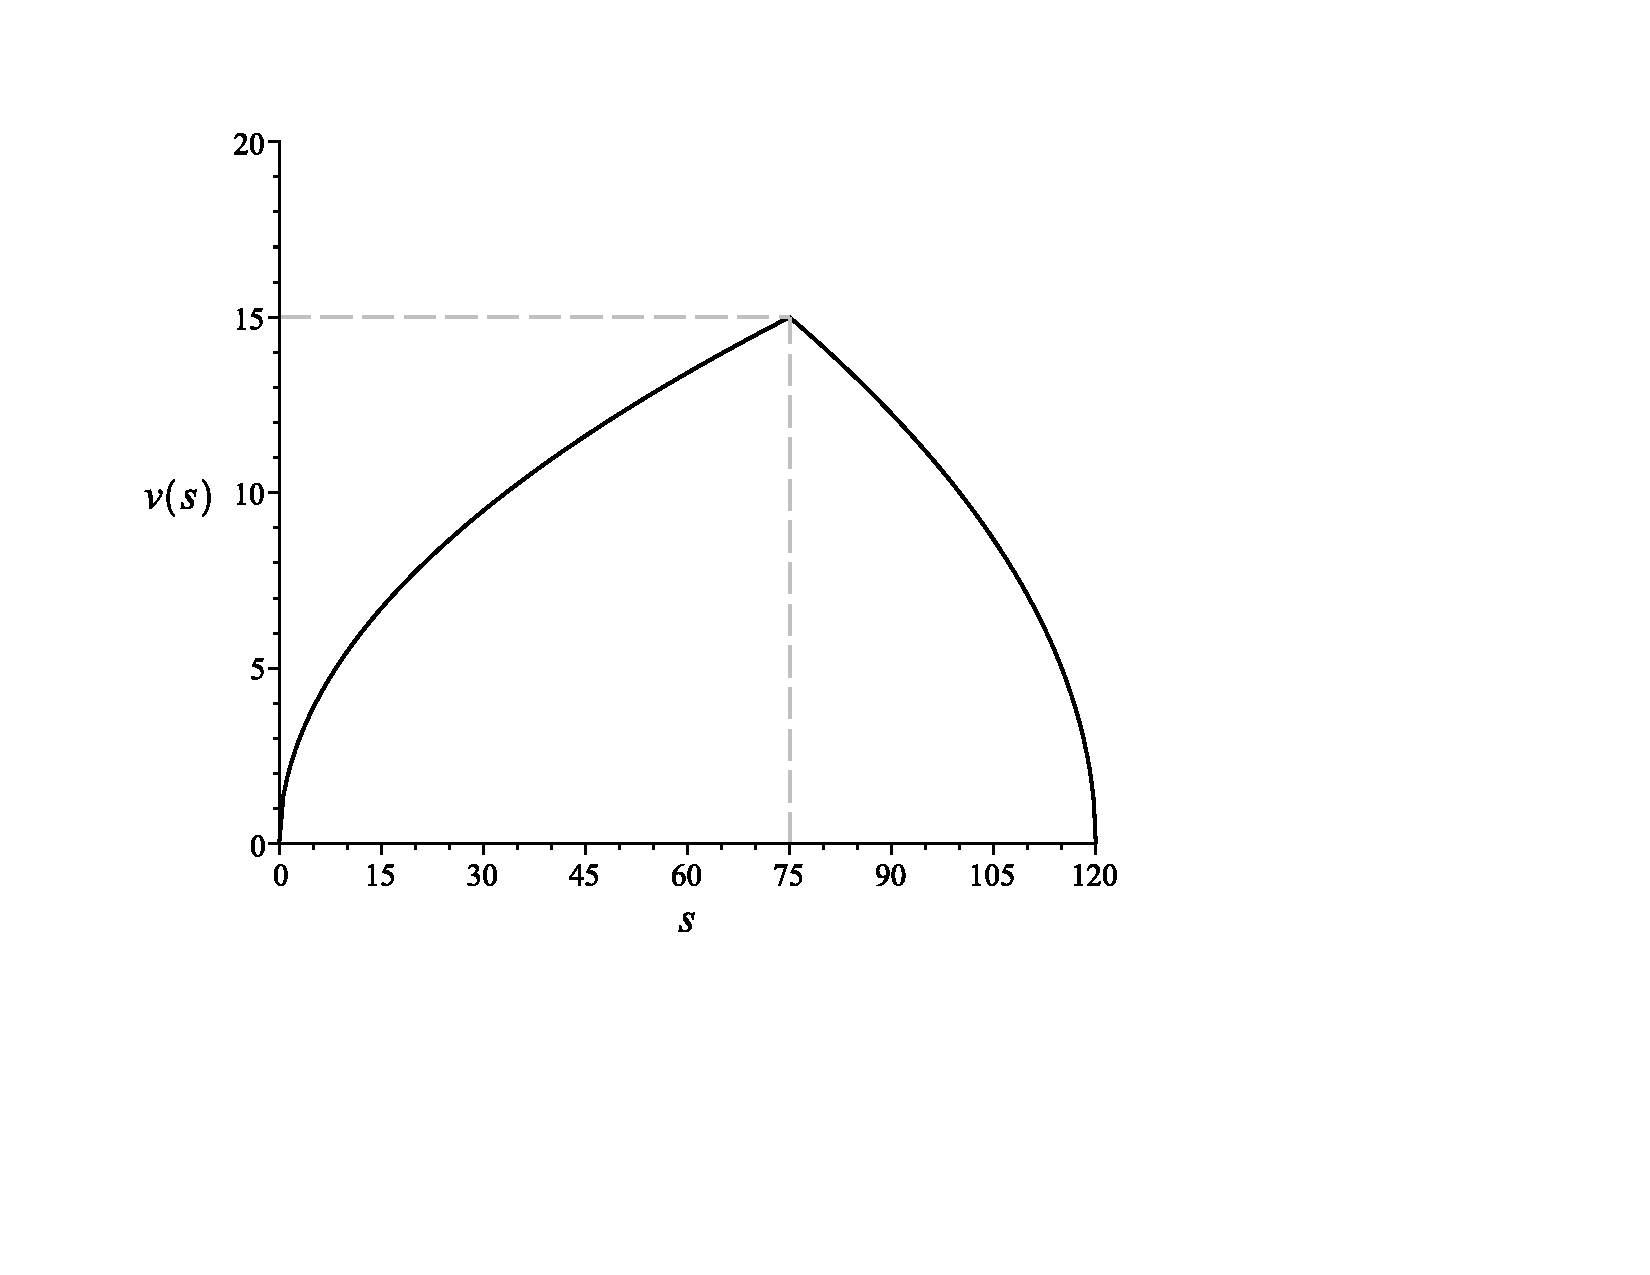
\includegraphics[scale=0.4]{v(s).pdf}
            \end{figure}
		  }
		%
      \end{enumerate}
	%
    %	
  \end{enumerate}
}

\multiproblem{huh2}{ A projectile is fired off a a cliff of height 5 m at a speed of 5 ms$^{-1}$
	%
		\begin{center}
		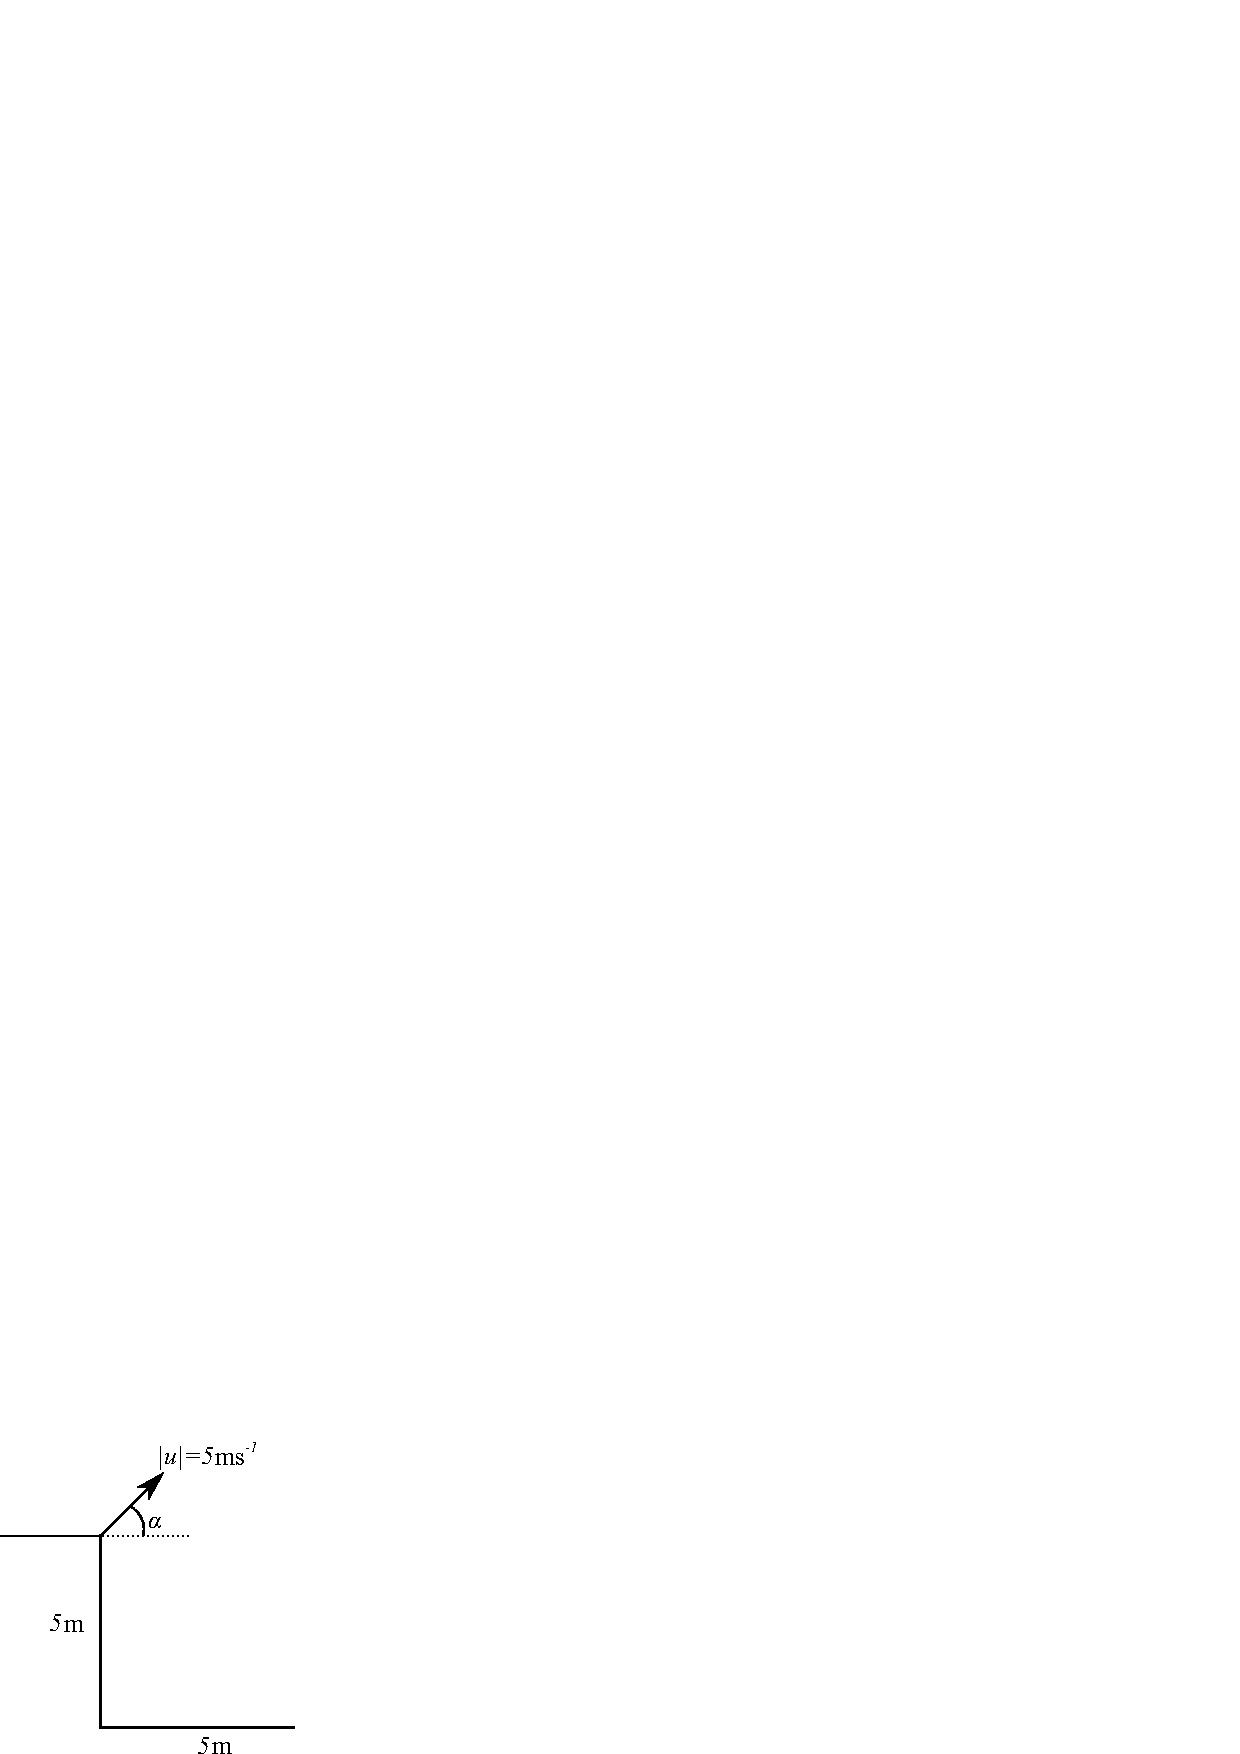
\includegraphics[]{cliff.pdf}
		\end{center}
	%
	\begin{enumerate}
    	%
		\item{ 	At what angle from the horizontal $\alpha$ must the projectile be fired in order for it to land 5m from the base of the cliff?\A{\\
			$\underline{s}=(5,-5)^{T}$, $\underline{u}=(5\cos \alpha,5\sin \alpha)^{T}$ and $\underline{a}=(0,-g)^{T}$. Using S(2) vertically and horizontally, we can solve for $\alpha$.\\
			Horizontally:\\
			$s_x=5=5 \cos \alpha t$, so $t=\sec \alpha$ \\
			Vertically:\\
			$s_y=-5=5\sin \alpha t -\frac{1}{2}g t^2$\\
			Substituting our result for $t$:
			$-5=5\sin \alpha \sec \alpha -\frac{1}{2}g \sec^2 \alpha$\\
			$-5=5 \tan \alpha -5 \sec^2 \alpha=5 \tan \alpha -5 (1+\tan^2 \alpha)$\\
			$0=\tan \alpha-\tan^2 \alpha$\\
			So either $\tan \alpha=0$ or $\tan \alpha =1$. And so, $\alpha=0$ or $\alpha=45^o=\pi/4$ radians respectively.}}
		%
		\item{Sketch the trajectory/trajectories found in (a) \A{ \\
				\begin{center}
					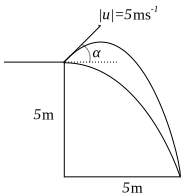
\includegraphics[]{cliff_traj.pdf}
				\end{center}
				}
		}
		%
		\item{ At what angle must the projectile be fired in order to be in the air for 1 second? \A{ \\We can simply look at the projectile's motion vertically, $s_y=-5=5 \sin \alpha \times 1 -\frac{1}{2}g \times 1$. So
			$0=\sin \alpha$. Looking at the configuration, the correct solution is $\alpha=0$}}
		%
		\item{For general $\alpha$ find an expression for the distance of the projectile from its initial position as a function of time $t$ \A{\\
			$s_x=5t\cos \alpha$ and $s_y=5t\sin \alpha - 5t^2$. The distance can be found by $d=\sqrt{s_x^2+s_y^2}$\\
			$d=\sqrt{25t^2 \cos^2 \alpha + 25t^2 \sin^2 \alpha - 50 t^3 \sin \alpha +25t^4}$\\
			$d=5t\sqrt{1 - 2t \sin \alpha +t^2}$ for $t\geq0$}} 
		%
	\end{enumerate}
}


\multiproblem{huh3}{A projectile is fired off a a cliff of height $h$, onto a hill, with an initial velocity of $$\underline{u}=(u,0)^{\mathrm{T}} \mathrm{ms}^{-1}$$\\
	%
		\begin{center}
		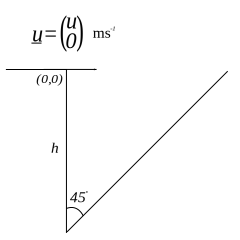
\includegraphics[]{cliff_hill.pdf}
		\end{center}
	%
	\begin{enumerate}
		%
		\item{ 	Show that the time in the air is $$T=\frac{-u+\sqrt{u^2+2gh}}{g}$$. \A{\\The vertical displacement is given by $s_y=-\frac{1}{2} gt^2$ the horizontal $s_x=ut$\\
			We know that at the impact at $t=T$, $s_y=h-s_x$, so\\
			(1)     $s_x=uT$\\
			(2)     $s_x-h=-\frac{1}{2}gT^2$\\
			(1)-(2) $h=uT+\frac{1}{2}gT^2$\\
			Solving for $T$, we find $$T=\frac{-u\pm\sqrt{u^2 +2gh}}{g}$$.\\
			We want the positive time solution, so $$T=\frac{-u+\sqrt{u^2 +2gh}}{g}$$.}
		}
		%
		\item{Using the previous result, find the position vector at which the projectile hits the slope as a function of $h,u$ and $g$.\A{\\We found that $s_x=ut$ so at impact $$s_x=uT=\frac{-u^2+u\sqrt{u^2 +2gh}}{g}$$\\
			Furthermore, on the slope, we have that $$s_y=s_x-h=\frac{-u^2+u\sqrt{u^2 +2gh}}{g}-h$$ So the position vector  is given by 
			$$\underline{p}_I=\left(\frac{-u^2+u\sqrt{u^2 +2gh}}{g},\frac{-u^2+u\sqrt{u^2 +2gh}}{g}-h\right)^T$$.\\ N.B. $^T$ does not mean ``to the power of time $T$'' but the transpose.}
		}
		%
		\item{ What are the limit of this position as $u\to \infty$ and $u\to 0$ \A{ \\
			This can either be found by intuition, or by mathematically finding the limits.\\
			\textit{Intuitively}, as $u\to \infty$ the time taken to reach the slope tends to zero, and so the distance the projectile falls tends to zero (at a faster rate $s_y=\mathcal{O}(t^2)$ ). Therefore we can deduce that the position vector $\underline{p}\to (h,0)^T$.\\
			As $u\to 0$ the projectile can be considered as simply falling vertically, and so the distance the projectile travels horizontally tends to zero. We know that $s_y=s_x-h$, therefore we can deduce that the position vector $\underline{p}\to (0,-h)^T$.\\
			\textit{Mathematically}, the limit as $u\to 0$ can also be found in a few ways. We can find that the limit as $T\to0$ is finite $\sqrt{2h/g}$ and so $s_x=uT\to0$. We can then trivially find $\underline(p)\to(-h,0)^T$.
			The limit as $u\to \infty$ is far harder. Let us start by rearranging $$s_x=\frac{-u^2+u\sqrt{u^2 +2gh}}{g}=\frac{u^2}{g}\left(-1+\sqrt{1+\frac{2gh}{u^2}}\right)$$
			Now we need the expansion $$(1+z)^a=1+az+\frac{a(a-1)}{2!}z^2+...$$
			In the case where $a=\frac{1}{2}$
			$$(1+z)^\frac{1}{2}=1+\frac{1}{2}z-\frac{1}{8}z^2+...$$
			So
			$$s_x=\frac{u^2}{g}\left(-1+\left(1+\frac{1}{2}\frac{2gh}{u^2}-\frac{1}{8}\left(\frac{2gh}{u^2}\right)^2+...\right)\right)$$
			$$s_x=h-\frac{gh^2}{4u^2}+\mathcal{O}(u^{-4})...$$
			Therefore, the limit as $u\to\infty$ of $s_x=h$.}
		}
		%
		\item{Find an expression for the distance of the projectile from its initial position as a function of time $t$\A{ \\
			$s_x=ut$ and $s_y=- \frac{1}{2}gt^2=-5t^2$. The distance can be found by $d=\sqrt{s_x^2+s_y^2}$\\
			$d=\sqrt{u^2 t^2    +25t^4}$\\
			$d=ut\sqrt{1  +\left(\frac{5t}{u}\right)^2}$ for $t\geq0$}
		} 
		%
	\end{enumerate}
}

\multiproblem{huh4}{ 
	I am throwing a ball up to a friend on top of a roof 20 m above me.
	\begin{enumerate}
		%
		\item{What is the minimum initial velocity with which I can throw the ball, so that it reaches my friend?\A{\\
			Intuitively, at the highest point the ball reaches, its veritcal component of the velocity must be equal to zero. 
			So using $v^2=u^2+2as$ we can rearange to find $s_{\mathrm{max}}=\frac{u^2}{2g}$. 
			If we need the ball to reach 20 \metres, $s_{\mathrm{max}}=\frac{u^2}{2g}\geq20$. 
			Therfore, $u\geq\sqrt{40g}$, and $u_{\mathrm{min}}=20$\mps }
		}
		%
		\item{I now need the ball to reach my friend within 1 second. What is the minimum initial velocity with which I can throw the ball now? \A{\\
			We have $s$, $a$, $t$ and want to find $u$. Rearranging $s=ut+\frac{1}{2}at^2$, we find $u=\frac{s-\frac{1}{2}at^2}{t}=25 \mps$.\\
			It is interesting to note that there is only one solution. Why is this?\\
			Let us check our result by taking a slightly different approach. We can find $20=ut-5t^2$, solving for $t$, $t_\pm=\frac{u\pm\sqrt{u^2-400}}{10}$.\\
			Clearly $u > \sqrt{u^2-400}$ for $u\geq20$ and so there are two positive solutions for $t$.\\
			Let us choose the smaller solution and equate it to our desired time, $1=\frac{u-\sqrt{u^2-400}}{10}$\\
			We can the find that $u=25\mps$.\\
			Is it possible for the ball to pass my friend twice within 1 second?\\
			We can find this by looking at the larger solution to $t$, $T=\frac{u+\sqrt{u^2-400}}{10}$. 
			This solution (where it exists) is always greater than $u/10$. The minimum velocity with which the ball can be thrown and it still reach my friend is $20$\mps. Therefore this second time is always greater than 2 seconds. 
			The ball cannot pass my friend twice within 1 second. 		
			}}
		%
		\item{If my friend misses the first opportunity to catch the ball, how long is it before they get another chance?\A{\\
			We found that the times at which the ball could pass my friend were given by $t=\frac{u\pm\sqrt{u^2-400}}{10}$.\\
			Furthermore, when $u=25\mps$ the first solution $t_-=1$. The second solution $t_+= \frac{25+\sqrt{225}}{10}=4$ seconds. Therefore the time between opportunities to catch is 3 seconds. }}
		%
		\item{How quickly would I have to throw the ball to reach my friend if they were at a height $h$ in order to reach them within 1 second?\A{\\
			$h=ut-5t^2$ and so $u=h+5$\mps.}}
		%
		\item{If my friend misses the first catch, how long before they have another opportunity to catch it now?\A{\\
			$t_\pm=\frac{h+5\pm \sqrt{(h+5)^2-20h}}{10}=\frac{(h+5)\pm(h-5)}{10}$. The time between the opportunities is therefore $t_+ -t_-=\frac{h}{5}-1$ seconds. }} 
		%
	\end{enumerate}
}

\multiproblem{huh5}{
	This question deals with deriving the SUVAT equations. In general the differential equations relating displacement, velocity and acceleration of a body are given by $\frac{ds(t)}{dt}=v(t)$, and $\frac{dv(t)}{dt}=a(t)$.
	%
	\begin{enumerate}
		%
		\item{Using these, and the fact that we are modeling a situation where the acceleration is constant, derive an expression for $v(t)$ and one for $s(t)$ by integration. (Your solutions will look slightly different to S(1) and S(2), briefly explain this difference).  \A{ \\
		Constant acceleration implies $a(t)=a$, so by integrating both sides of $\frac{dv(t)}{dt}=a$ w.r.t. $t$ we find $v(t) = v(0) + at$.\\
		If we now substitute this into the RHS of $\frac{ds(t)}{dt}=v(t)$, and integrate again, we find $s(t)=s(0)+v(0)t+\frac{1}{2}at^2$.\\
		We usually denote the initial velocity $u:=v(0)$, and in general in SUVAT equations we assume initial displacement $s(0)=0$, giving us exactly S(1) and S(2).}}
		%
		\item{Using your answers from (a), derive S(5). \A{ \\
		Rearrange S(1) to $u=v-at$. Now substitute this into S(2), giving $s=(v-at)t+\frac{1}{2}at^2=vt-\frac{1}{2}at^2$.}}
		%
		\item{Using separation of variables, show that the area under a velocity-time plot (the graph of $v(t)$) is equal to the displacement. Is this result valid even for non-constant acceleration? \A{ \\
		Starting with $\frac{ds(t)}{dt}=v(t)$, mulitply both sides by $dt$ and integrate, $\int ds = \int v(t) dt$. \\
		Since the LHS is just $s(t)$, this tells us that displacement is equal to the area under the graph of $v(t)$. \\
		Nowhere have we implictly used constant acceleration, and this result is true for non-constant acceleration too, meaning $v(t)$ could be any curve, not just straight lines.}}
		%
		\item{Constant acceleration implies constant gradient on a velocity-time plot, use this and a sketch to verify S(3). \A{ \\
		From a simple veolcity time graph with constant acceleration, we can see that the area under $v(t)$ will always be a trapezium (or a trinagle if $u=0$). \\
		Hence we can find this area by taking the average of the two endpoints, which are at $u$ and $v$ over $t$. Or we can just find it geomtrically. This gives us $s=\frac{1}{2}(u+v)t$.}}
		%
		\item{From Newton's First Law, constant acceleration implies constant force acting on the body. Write down expressions for work done and kinetic energy, and hence derive S(4). (You will need to use the fact that work done is equal to the change in kinetic energy) \A{ \\
		The scalar expression for work done is $W=Fs$, and for the kinetic energy of a body with mass $m$ is $E_k=\frac{1}{2}mv^2$. \\
		Using the fact that work done can be measured as the change in kinetic energy of a body $W=\Delta E_k$, we can see the work done taking the body from initial velocity $u$ to final velocity $v$ is $W=\frac{1}{2}m\Delta v^2=\frac{1}{2}m(v^2-u^2)$ in SUVAT notation. \\
		We also know $W=(ma)s$ using Newton. \\
		Equating these two expressions for work done, $2mas=m(v^2-u^2)$, dividing through by m and rearranging gives S(4).}
		}
	\end{enumerate}
}

\multiproblem{huh6}{ 
	\begin{enumerate}
		\item{In an experiment I drive a car, mass $m$, from stationary to a flag 20m away applying constant acceleration of 4\mpssq. Find the time $t^*$ it takes me to reach the flag. \A{ \\
		We use $s=ut+\frac{1}{2}at^2$ with $u=0$, $s=20$, $t=t^*$ and $a=4$, to find $t^*=\sqrt{10}$.}}
		%
		\item{I repeat the experiment, but this time I see a hazard in the distance at time $\tau<t^*$ and immediately apply constant deceleration. Find an expression for $F$, the force required to bring the car to a stop at the flag, as a function of $\tau$. Sketch the graph of $F(\tau)$. \A{ \\
		We begin by finding expressions for the car's velocity and displacement at time $\tau$, just before the deceleration is applied. We use a subscript 1 to denote quantities before deceleration, and subscript 2 for after. \\
		Using the same equation as above we find $s_1=\frac{1}{2}(4\tau^2)=2\tau^2$. From $v_1=u_1+a_1t$ with $u_1=0$ we have $v_1=2\tau$. \\
		Now, we need to find the force applied to get the car to stop. This means we need the acceleration applied after $\tau$, $a_2$. Our initial velocity is the final velocity from before $u_2=v_1=2\tau$. \\
		Since we need to come to a stop at the flag 20m away, and we've already travelled a distance of $s_1$, we have $s_2=20-s_1=20-2\tau^2$. Also, since we come to a stop, $v_2=0$.
		Now using $v_2^2=u_2^2+2a_2s_2$, we have $0=16\tau^2+2a_2(20-2\tau^2)$. Rearranging this gives $$a_2=\frac{-16\tau^2}{4(10-\tau^2)}.$$ \\
		The force required is directly proportial to this so we find, $$F(\tau)=\frac{-4m\tau^2}{10-\tau^2}.$$\\
		This is singular for $\tau=\sqrt{10}$ (our answer from the first part) because as $\tau$ approaches that time, the force required to stop the care in such a small amount of time tends to infinity.
		}}
		%
		\item{In another experiment, I drop a coin down a well which has a depth of 75\metres. Assuming the speed of sound is 300\mps, find the time at which I hear the coin hit the bottom. \A{ \\
		First we find the time taken for the coin to hit the bottom of the well using $s=ut+\frac{1}{2}at^2$, with $u=0$, $a=g$ and $s=75$, giving $t=5\sqrt{6/g}$.
		The time taken for the sound to travel up the well to me, call it $t_s$, is found using the formula for constant velocity ($v_s=s/t_s$), where $v_s$ is the speed of sound. Giving $t_s = 0.25$. \\
		Adding these two results together gives the answer, $T=5\sqrt{6/g}+\frac{1}{4}$.
		}} 	
	\end{enumerate}}


\multiproblem{huh7}{  This question concerns a popular firework device which can fire fireworks out at any angle to the horizontal. We treat these fireworks as projectiles with initial speed $u$ under acceleration due to gravity $g$. We want to find an analytic expression for the boundary of the `safe area', where no firework can reach.
	\begin{enumerate}
		\item{Write down $\mathbf{u}=(u_x,u_y)$, the firework's initial velocity as an expression in $\theta$, the angle at which the firework is fired from. \A{ \\
		Using trigonometry we can split the initial veolicty into vertical and horizontal components: $(u_x, u_y) = (u\cos(\theta), u\sin(\theta))$.}
		}
		%
		\item{If $\big(s_x(t), s_y(t)\big)$ is a firework's position at time $t$, show that the graph of a firework's trajectory is
		\begin{equation}
			s_y = s_x \tan\theta - \frac{s_x^2g}{2v^2}\big(1+\tan^2\theta\big).
		\end{equation}
		\textit{Hint: Begin by finding $s_x$ and $s_y$ and then relate them by explicitly eliminating $t$.} \A{ \\
		We use the vector form of $s=ut+\frac{1}{2}at^2$, with $(u_x,u_y)$ as above and $(a_x,a_y)=(0,g)$. We find $$s_x = ut\cos(\theta)$$ $$s_y=ut\sin(\theta)+\frac{1}{2}gt^2.$$ \\
		Rearranging the first equation we have $t=\frac{s_x}{u\cos(\theta)}$, substituting this into our equation for $s_y$ we can eliminate any explicit dependence on $t$, to give, $$s_y = s_x \tan(\theta) + \frac{g}{2}\Big(\frac{s_x^2}{u^2\cos^2(\theta)}\Big).$$ \\
		Then using the fact that $\frac{1}{\cos^2(\theta)}=\text{sech}^2(\theta)=1+\tan^2(\theta)$, $$s_y = x\tan(\theta)+\frac{gs_x^2}{2gu^2}\Big(1+\tan^2(\theta)\Big),$$ as required. \\
		It's important at this point to understand what this solution is. If we choose one particular value, $\theta=\theta'$, the graph of $s_y(s_x, \theta')$ is the trajectory of the firework fired at angle $\theta'$, which will be a parabola. Of course then if we choose a particular $s_x$ then we would find a position along this trajectory $(s_x,s_y)$.
		}}
		%
		\item{This equation is the family of all possible firework trajectories. You can think of it as $s_y$ as a function of $s_x$, parametrised by a choice of $\theta\in[0,\pi]$. In other words for a particular choice of $\theta$, the graph of $s_y(s_x)$ is that firework's trajectory. Now, we want to maximise this set over $\theta$. Find $\frac{\partial s_y}{\partial \theta}$ and hence find the maximal $s_y$ position for any given $s_x$ position.
		\textit{Hint: Instead, use the substitution $z=\tan\theta$ and maximise $s_y(s_x)$ with respect to $z$. Bonus question: think why this substitution is allowed by considering the graph of $\tan(\theta)$.} \A{ \\
		From here, it is useful to consider $s_y$ as a multivariate function in $s_x$ and $\theta$, $s_y(s_x,\theta)$. \\
		To maximise a function over its range we find where the derivative vanishes, then we can check to see if the function is locally maximal there by looking at the second derivative (curvature). \\
		For multivariate functions, such as this, we find where the relevant partial derivative vanishes. Using the substitution $z=\tan(\theta)$, we have $$s_y = s_x z + \frac{gs_x^2}{2u^2}(1+z^2)$$
		$$\frac{\partial y}{\partial z} = x + \frac{gzs_x^2}{u^2}.$$ Solving where this is zero is the turning point, we find it occurs where $z=z_{max}=-\frac{u^2}{gs_x}$, notice this is a function of $s_x$ but not $s_y$. We can check this is maximal by seeing the second partial derivative here is negative. \\
		By substituting this value for $z_{max}$ into equation our equation for $s_y$, we only consider a special `slice' through the function $s_y$ such that it is only dependent on $s_x$ and along which $s_y$ is maximal for any given $s_x$.\\
		So we denote $s_{max,y}(s_x):=s_y(s_x, z_{max})$ and find, $$s_{max,y} = -\frac{u^2}{g}+\frac{gs_x^2}{u^2}\Big(1+\Big(\frac{u^2}{gs_x}\Big)^2\Big) = \frac{1}{2}\Big(\frac{gs_x^2}{u^2}-\frac{u^2}{g}\Big).$$ \\
		The graph of $s_{max,y}(s_x)$ is our solution. If we choose a distance along the horizonal, $s_x=x$, this function gives us the maximal height, $s_{max,y}(x)$, that \textit{any} firework could reach above $x$. \\
		We could work out which firework it was that reached that height by solving $z_{max}(x)=\tan(\theta)$ for $\theta$. \\
		Every trajectory is a parabola, and what we've found is that their maximal boundary is also parabolic. \\
		(The substitution $z=\tan(\theta)$ is valid as $\tan(\theta)$ is monotically increasing between $[-\pi/2, \pi/2]$. This means that any turning points will be the same before and after the substitution.)
		}}
		%
		\item{Sketch the safe area boundary that you have found. \A{ \\
				\begin{center}
					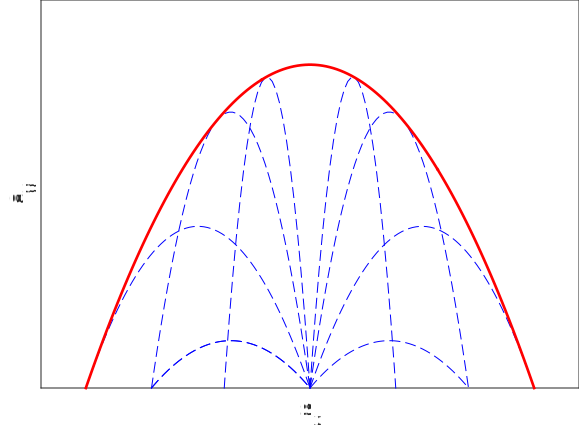
\includegraphics[scale=0.5]{safety_envelope.pdf}
				\end{center}
			This shows a few sample trajectories, for different values of $\theta$ in dashed blue, then the safety boundary in red. Notice how it is tangent to the trajectories, but not at their own maxima.}
		}
		%
	\end{enumerate}
}
